\section{Robustness tests}
\label{sec:robustness}
% =====================================================================

We test the sensitivity of the measurements to the numerical choices on the first 8 subvolumes of the fiducial catalogue (line of sight $z$). Each test is repeated for both methods, and the change of the Q1 and Q4 cross-correlation monopoles is expressed in units of the statistical error of one subvolume (Figure~\ref{fig:robustness}).

\paragraph{Periodic padding.} Increasing the padding around each subvolume from 30 to $60\Mpch$ leaves the ASTRA values of $r$, and therefore all the statistics, unchanged: the Delaunay neighbourhood of every point of the subvolume is already contained in the $30\Mpch$ padding.

\paragraph{Number of randoms.} Doubling the number of random points in the tessellation ($N_r=2N_g$) shifts the ASTRA Q1 cross-correlations by up to $4\sigma$ and the Q4 ones by up to $2\sigma$ at $s\lesssim40\Mpch$, while density split, for which the randoms are only query points, changes by less than $0.2\sigma$. In ASTRA the randoms enter the definition of $r$ itself (Eq.~\ref{eq:astra_r}), so $N_r/N_g$ is a parameter of the statistic and must be kept fixed.

\paragraph{Sampling density.} Randomly thinning the galaxies (and the randoms in the same proportion) by a factor 2 (5) shifts the ASTRA random-quartile cross-correlations by 7--8 (22)$\sigma$ at $s\simeq20$--$40\Mpch$, and up to 12 (40)$\sigma$ for the galaxy Q1, against $\sim1$ (3--5)$\sigma$ for density split. At the level of individual points, the rank correlation between the $r$ of the same galaxies computed in the full and in the thinned samples is only $0.65$, $0.38$ and $0.24$ for thinning factors of 2, 5 and 10, and only 58\%, 43\% and 36\% of the galaxies of the extreme quartiles keep their quartile.

This is an intrinsic property of the estimator rather than a numerical instability. ASTRA is an \emph{adaptive-scale} statistic: the environment of a point is defined by its Delaunay neighbours, so its effective scale is the typical distance between neighbours, $\propto\bar n^{-1/3}$, and it changes with the sampling density. Thinning enlarges this scale, which is why the changes are concentrated at $s\lesssim50\Mpch$, whereas density split keeps a fixed smoothing radius. This is not a limitation for the present analysis or for DESI, since the density is fixed in the mocks as in the data (and in an emulator trained at that density). It implies however that ASTRA statistics must be compared, modelled and emulated at the same number density and random-to-galaxy ratio, and that comparisons with density split must be made at equal density, as throughout this paper.

\begin{figure*}[!tp]
\centering
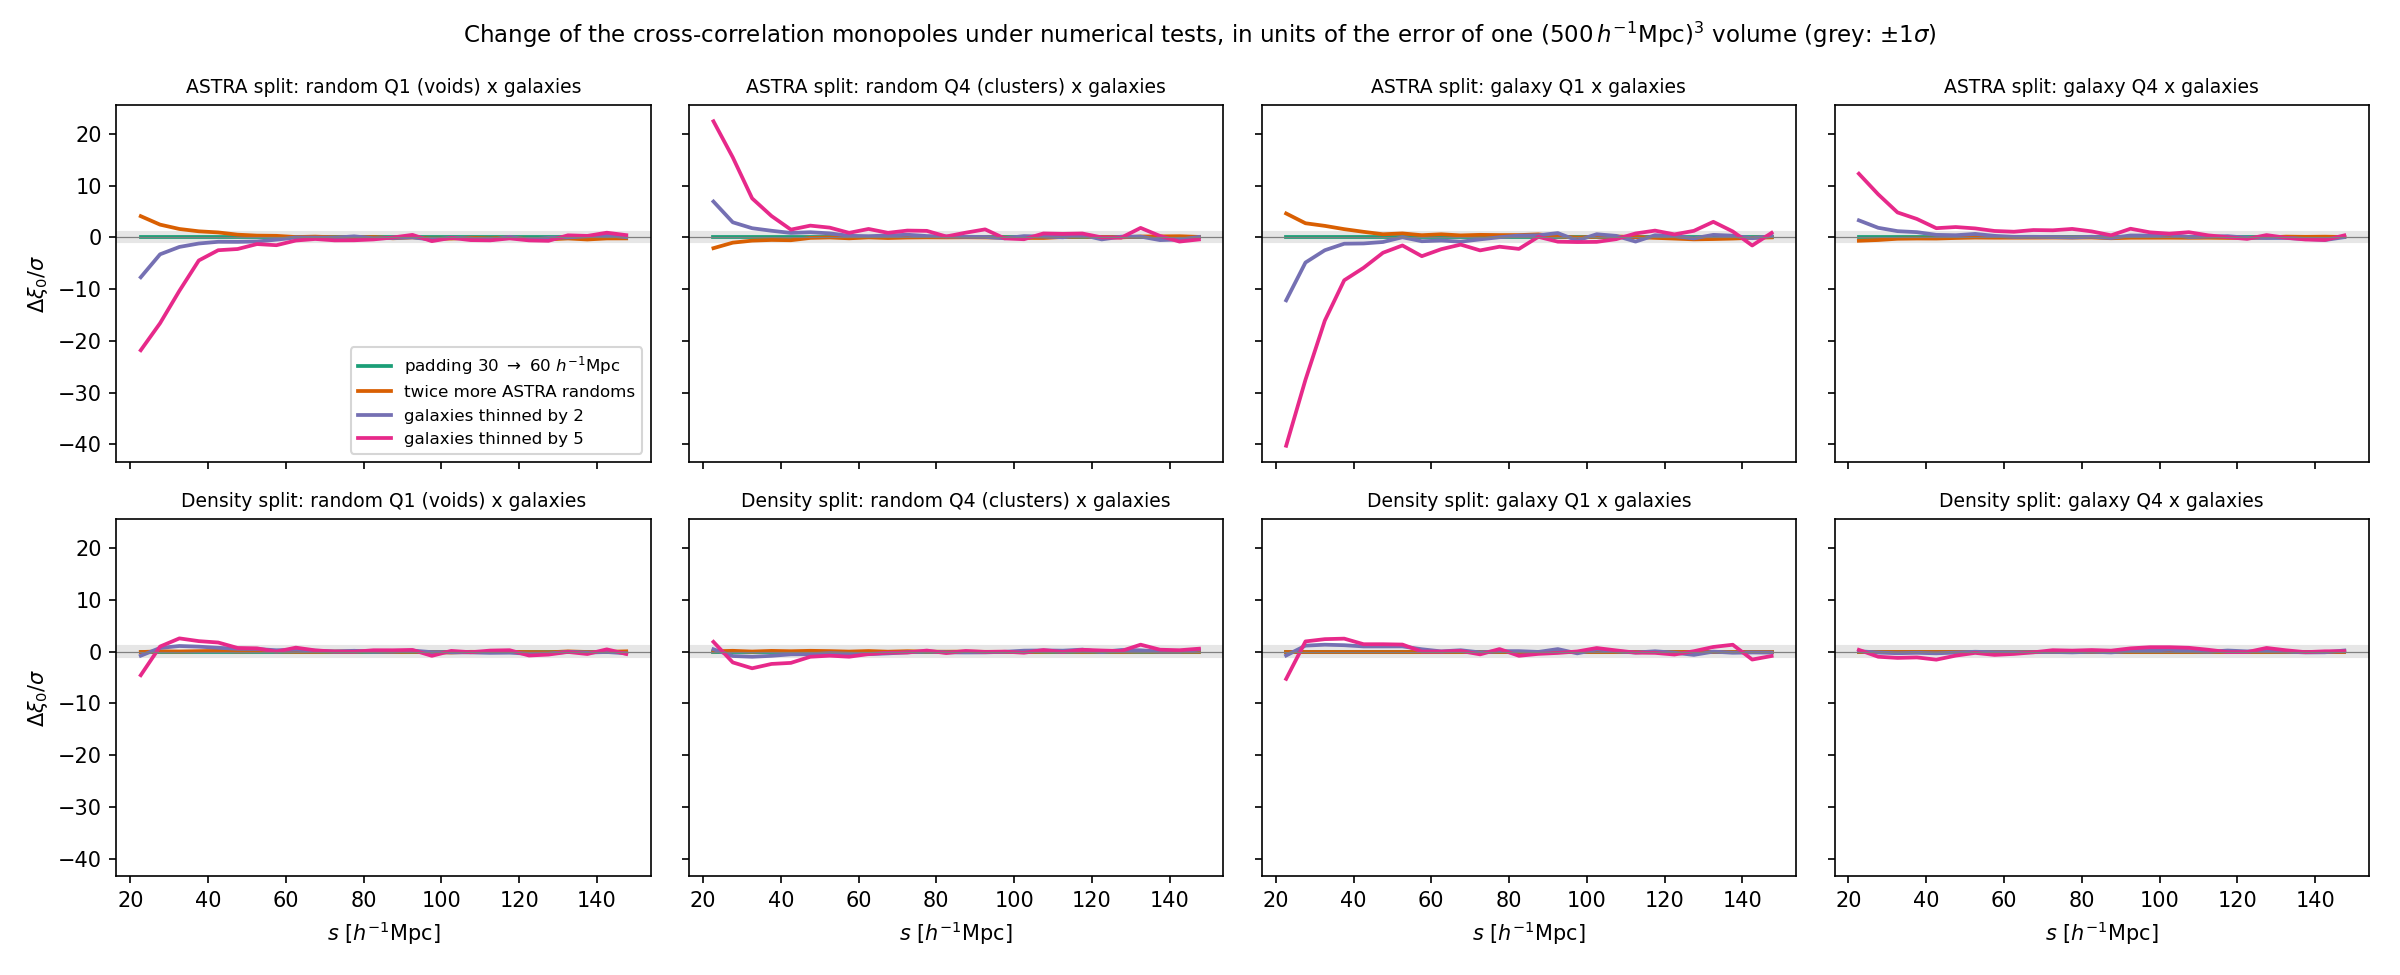
\includegraphics[width=\textwidth]{readable_robustness.png}
\caption{Change of the Q1 and Q4 cross-correlation monopoles (random quartiles, left; galaxy quartiles, right) of ASTRA split (top) and density split (bottom) when the padding is doubled (green), the ASTRA randoms are doubled (orange), and the galaxies are thinned by 2 (purple) and 5 (pink), relative to the baseline, in units of the error of one $(500\Mpch)^3$ volume (grey band: $\pm1\sigma$). Mean over 8 subvolumes of the fiducial catalogue.}
\label{fig:robustness}
\end{figure*}


